\documentclass{standalone}
\usepackage{tikz}
\usetikzlibrary{patterns, positioning}
\usetikzlibrary{shapes.misc}
\usepackage[outline]{contour}
\contourlength{1.5pt} 


\begin{document}
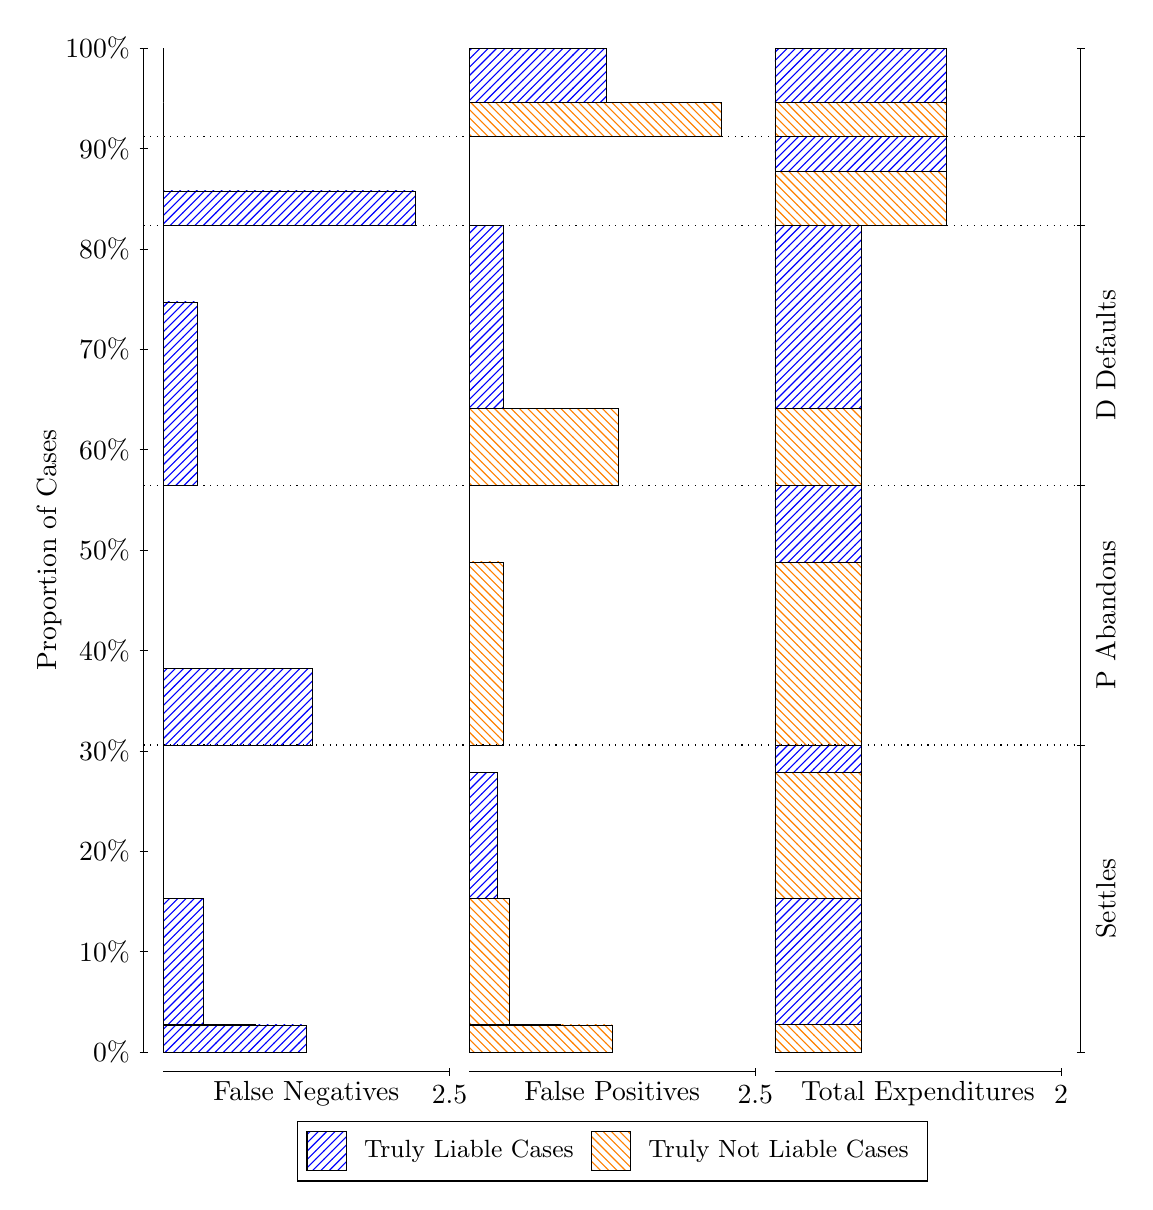
\begin{tikzpicture}
\draw[black, very thin] (1.5,1.75) -- (1.5,14.5);
\node[rotate=90, text=black, anchor=center] at (0.3, 8.125) {Proportion of Cases};
\draw[black, very thin] (1.45,1.75) -- (1.55,1.75);
\node[text=black, anchor=east] at (1.45, 1.75) {0\%};
\draw[black, very thin] (1.45,3.025) -- (1.55,3.025);
\node[text=black, anchor=east] at (1.45, 3.025) {10\%};
\draw[black, very thin] (1.45,4.3) -- (1.55,4.3);
\node[text=black, anchor=east] at (1.45, 4.3) {20\%};
\draw[black, very thin] (1.45,5.575) -- (1.55,5.575);
\node[text=black, anchor=east] at (1.45, 5.575) {30\%};
\draw[black, very thin] (1.45,6.85) -- (1.55,6.85);
\node[text=black, anchor=east] at (1.45, 6.85) {40\%};
\draw[black, very thin] (1.45,8.125) -- (1.55,8.125);
\node[text=black, anchor=east] at (1.45, 8.125) {50\%};
\draw[black, very thin] (1.45,9.4) -- (1.55,9.4);
\node[text=black, anchor=east] at (1.45, 9.4) {60\%};
\draw[black, very thin] (1.45,10.675) -- (1.55,10.675);
\node[text=black, anchor=east] at (1.45, 10.675) {70\%};
\draw[black, very thin] (1.45,11.95) -- (1.55,11.95);
\node[text=black, anchor=east] at (1.45, 11.95) {80\%};
\draw[black, very thin] (1.45,13.225) -- (1.55,13.225);
\node[text=black, anchor=east] at (1.45, 13.225) {90\%};
\draw[black, very thin] (1.45,14.5) -- (1.55,14.5);
\node[text=black, anchor=east] at (1.45, 14.5) {100\%};

\draw[black, very thin] (13.4,1.75) -- (13.4,14.5);
\draw[black, very thin] (13.35,1.75) -- (13.45,1.75);
\node[anchor=west] at (13.35, 1.75) {};
\draw[black, very thin] (13.35,5.6487) -- (13.45,5.6487);
\node[anchor=west] at (13.35, 5.6487) {};
\draw[black, very thin] (13.35,8.9485) -- (13.45,8.9485);
\node[anchor=west] at (13.35, 8.9485) {};
\draw[black, very thin] (13.35,12.249) -- (13.45,12.249);
\node[anchor=west] at (13.35, 12.249) {};
\draw[black, very thin] (13.35,13.374) -- (13.45,13.374);
\node[anchor=west] at (13.35, 13.374) {};
\draw[black, very thin] (13.35,14.5) -- (13.45,14.5);
\node[anchor=west] at (13.35, 14.5) {};

\draw[black, very thin, pattern color=blue, pattern=north east lines] (1.75,1.75) rectangle (3.5667,2.0945);
\draw[black, very thin, pattern color=blue, pattern=north east lines] (1.75,2.0945) rectangle (2.9127,2.1009);
\draw[black, very thin, pattern color=blue, pattern=north east lines] (1.75,2.1009) rectangle (2.2587,3.6992);
\draw[black, very thin, pattern color=orange, pattern=north west lines] (1.75,3.6992) rectangle (1.75,5.6487);
\draw[black, very thin, pattern color=blue, pattern=north east lines] (1.75,5.6487) rectangle (3.6393,6.6221);
\draw[black, very thin, pattern color=orange, pattern=north west lines] (1.75,6.6221) rectangle (1.75,8.9485);
\draw[black, very thin, pattern color=blue, pattern=north east lines] (1.75,8.9485) rectangle (2.186,11.275);
\draw[black, very thin, pattern color=orange, pattern=north west lines] (1.75,11.275) rectangle (1.75,12.249);
\draw[black, very thin, pattern color=blue, pattern=north east lines] (1.75,12.249) rectangle (4.9473,12.685);
\draw[black, very thin, pattern color=orange, pattern=north west lines] (1.75,12.685) rectangle (1.75,13.374);
\draw[black, very thin, pattern color=orange, pattern=north west lines] (1.75,13.374) rectangle (1.75,13.811);
\draw[black, very thin, pattern color=blue, pattern=north east lines] (1.75,13.811) rectangle (1.75,14.5);
\draw[black, very thin, pattern color=orange, pattern=north west lines] (5.6333,1.75) rectangle (7.45,2.0944);
\draw[black, very thin, pattern color=orange, pattern=north west lines] (5.6333,2.0944) rectangle (6.796,2.1008);
\draw[black, very thin, pattern color=orange, pattern=north west lines] (5.6333,2.1008) rectangle (6.142,3.6995);
\draw[black, very thin, pattern color=blue, pattern=north east lines] (5.6333,3.6995) rectangle (5.9967,5.2978);
\draw[black, very thin, pattern color=blue, pattern=north east lines] (5.6333,5.2978) rectangle (5.6333,5.6487);
\draw[black, very thin, pattern color=orange, pattern=north west lines] (5.6333,5.6487) rectangle (6.0693,7.9751);
\draw[black, very thin, pattern color=blue, pattern=north east lines] (5.6333,7.9751) rectangle (5.6333,8.9485);
\draw[black, very thin, pattern color=orange, pattern=north west lines] (5.6333,8.9485) rectangle (7.5227,9.922);
\draw[black, very thin, pattern color=blue, pattern=north east lines] (5.6333,9.922) rectangle (6.0693,12.249);
\draw[black, very thin, pattern color=orange, pattern=north west lines] (5.6333,12.249) rectangle (5.6333,12.938);
\draw[black, very thin, pattern color=blue, pattern=north east lines] (5.6333,12.938) rectangle (5.6333,13.374);
\draw[black, very thin, pattern color=orange, pattern=north west lines] (5.6333,13.374) rectangle (8.8307,13.811);
\draw[black, very thin, pattern color=blue, pattern=north east lines] (5.6333,13.811) rectangle (7.3773,14.5);
\draw[black, very thin, pattern color=orange, pattern=north west lines] (9.5167,1.75) rectangle (10.607,2.1008);
\draw[black, very thin, pattern color=blue, pattern=north east lines] (9.5167,2.1008) rectangle (10.607,3.7054);
\draw[black, very thin, pattern color=orange, pattern=north west lines] (9.5167,3.7054) rectangle (10.607,5.3041);
\draw[black, very thin, pattern color=blue, pattern=north east lines] (9.5167,5.3041) rectangle (10.607,5.6487);
\draw[black, very thin, pattern color=orange, pattern=north west lines] (9.5167,5.6487) rectangle (10.607,7.9751);
\draw[black, very thin, pattern color=blue, pattern=north east lines] (9.5167,7.9751) rectangle (10.607,8.9485);
\draw[black, very thin, pattern color=orange, pattern=north west lines] (9.5167,8.9485) rectangle (10.607,9.922);
\draw[black, very thin, pattern color=blue, pattern=north east lines] (9.5167,9.922) rectangle (10.607,12.249);
\draw[black, very thin, pattern color=orange, pattern=north west lines] (9.5167,12.249) rectangle (11.697,12.938);
\draw[black, very thin, pattern color=blue, pattern=north east lines] (9.5167,12.938) rectangle (11.697,13.374);
\draw[black, very thin, pattern color=orange, pattern=north west lines] (9.5167,13.374) rectangle (11.697,13.811);
\draw[black, very thin, pattern color=blue, pattern=north east lines] (9.5167,13.811) rectangle (11.697,14.5);
\draw[black, dotted] (1.5,5.6487) -- (13.4,5.6487);
\draw[black, dotted] (1.5,8.9485) -- (13.4,8.9485);
\draw[black, dotted] (1.5,12.249) -- (13.4,12.249);
\draw[black, dotted] (1.5,13.374) -- (13.4,13.374);
\draw[black, very thin] (1.75,1.5) -- (5.3833,1.5);
\node[text=black, anchor=north] at (3.5667, 1.5) {False Negatives};
\draw[black, very thin] (5.3833,1.45) -- (5.3833,1.55);
\node[text=black, anchor=north] at (5.3833, 1.45) {2.5};

\draw[black, very thin] (5.6333,1.5) -- (9.2667,1.5);
\node[text=black, anchor=north] at (7.45, 1.5) {False Positives};
\draw[black, very thin] (9.2667,1.45) -- (9.2667,1.55);
\node[text=black, anchor=north] at (9.2667, 1.45) {2.5};

\draw[black, very thin] (9.5167,1.5) -- (13.15,1.5);
\node[text=black, anchor=north] at (11.333, 1.5) {Total Expenditures};
\draw[black, very thin] (13.15,1.45) -- (13.15,1.55);
\node[text=black, anchor=north] at (13.15, 1.45) {2};

\node[text=black, centered, rotate=90] at (13.72, 3.6993) {\contour{white}{Settles}};
\node[text=black, centered, rotate=90] at (13.72, 7.2986) {\contour{white}{P Abandons}};
\node[text=black, centered, rotate=90] at (13.72, 10.599) {\contour{white}{D Defaults}};



\draw (7.449999999999999,1.5) node[draw=none] (baseCoordinate) {};
\begin{scope}[align=center]
        \matrix[scale=0.5, draw=black, below=0.5cm of baseCoordinate, nodes={draw}, column sep=0.1cm]{
            \node[rectangle, draw, minimum width=0.5cm, minimum height=0.5cm, pattern color=blue, pattern=north east lines] {}; &
            \node[draw=none, font=\small, text=black] (B) {Truly Liable Cases}; &
            \node[rectangle, draw, minimum width=0.5cm, minimum height=0.5cm, pattern color=orange, pattern=north west lines] {}; &
            \node[draw=none, font=\small, text=black] (B) {Truly Not Liable Cases}; \\
            };
\end{scope}

\end{tikzpicture}
\end{document}